Fast switching digital signals have a wide bandwidth that causes RF energy to be injected in the power supplies and radiated from that portion of the circuit.  Also, the high instantaneous current drawn by a switching digital signal can cause a voltage potential between the ground connections of the circuit and the ground at the power supply due to the non-zero resistance and inductance of ground planes, traces, and power supply leads.  Thus, it is desirable to have electrically isolated power and ground supplies for the analog and digital portions of the circuit.

Figure~\ref{fig:Ground} shows one possible power supply configuration of the RTSC and Electrophysiology Interface boards and shows analog (ASIG) and digital (DSIG) signal paths which connect an IC grounded to the analog plane (AGND) to a IC grounded by the digital ground plane (DGND).  The RTSC board is powered by the USB interface of the PC, which may or may not connect DGND to earth ground of the building electrical distribution system.  Digital signals from the FPGA are routed to the Electrophysiology Interface board over the Hirose FX2 connector, which also makes multiple connections between DGND on the Electrophysiology Interface board and the ground plane of the RTSC board.  The digital circuits on the Electrophysiology Interface board are powered by an isolated $+5.0\unit{V}$ fixed output bench-top power supply and are connected to the DGND plane.  The analog circuits are powered by the isolated variable outputs of the bench-top power supply and are connected to the AGND plane.  The AD5678 DAC is powered by the digital supply, and its analog output signals are connected to the differential output amplifier blocks that are powered by the analog supplies.  The AD7606 ADC communicates with the digital signals of the FPGA, and its IO buffers are powered by a digital supply, but its main power supply is analog.  The Preamp boards receive analog power from the PCI-Express connectors, and their digital signals are controlled by the CPLD powered by the digital supply.

\begin{figure}[h!]
	\centering 
		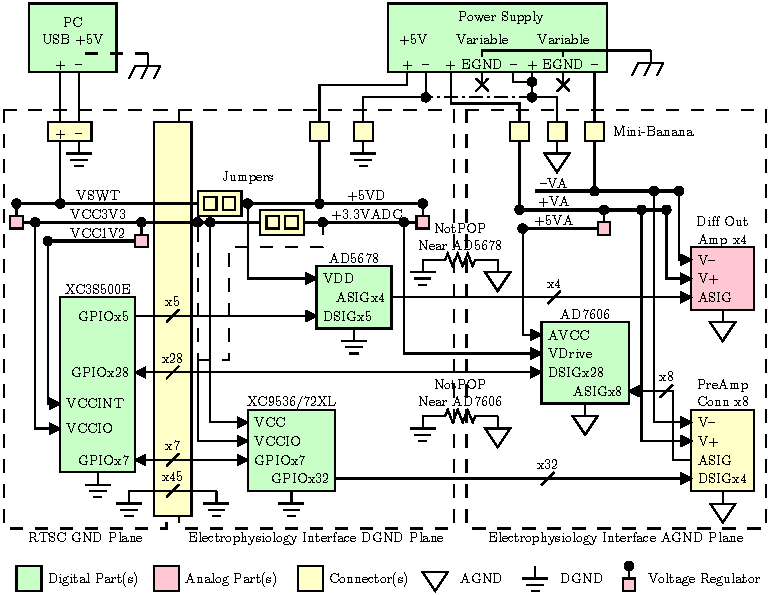
\includegraphics{./figures/Ground} 
	\caption{Ground planes\label{fig:Ground}}
\end{figure}

The communication between parts powered by the analog and digital supplies requires that the signals be referenced to a common node.  Thus, the analog and digital grounds are connected near the bench-top power supply.  This has the effect of minimizing ground-bounce by directing the current return of most of the fast switching digital signals through the digital power supply lead, but it directs the signal return current, from signals that cross the ground planes, to the bench-top power supply before it can return to the signal source, yielding a large signal loop that increases radiated emissions~\cite{Montrose1999}.

Both the AD5678 and AD7606 recommend that, if analog and digital ground connection is needed, it should be close to the the respective IC~\cite{AD7606ds,AD5678ds}.  Near the AD5678 and near the AD7606, pads for $0\unit{\Omega}$ resistors may be populated to allow a shorter signal current return path, but if multiple signals switch at once, the actual non-zero resistance of the resistor, via, and trace connecting the ground planes will be out of balance with the signal trace resistance and may allow signal return current in the ground planes to divert back to the bench-top power supply.

Future designs should consider suggestions in~\cite{Montrose1999} for completely isolating analog and digital power and ground using opto-isolators or isolation transformers for digital signals that need to communicate between analog and digital circuits, or an alternative is to bridge analog and digital planes under signals that interface with analog and digital circuits.
